 \documentclass[write-up.tex]{subfiles}
 \begin{document}
\section{Development and Testing}
%Talk about how the equation for the smoothing kernel changed to remove 15/(pi h^6) cuz values were too small, redo volume and derivatives as well as do some tweaking to find optimum values.
\subsection{Boilerplate code}

The beginning of my implementation involved the boilerplate minimal code required for my graphics library SFML to be setup as well as including key libraries I will need throughout the project.
\begin{lstlisting}

#include <SFML/System/Vector2.hpp>
#include <SFML/Graphics.hpp>
#include<iostream>
#include <algorithm>
#include<vector>
#include<cmath>
#include <omp.h>

int main()
{
    //Initialize SFML
    sf::RenderWindow window(sf::VideoMode(900, 900), "Smoothed Particle Hydrodynamics Simulation");
    window.setFramerateLimit(120);
    sf::View view = window.getDefaultView();
    sf::Vector2u window_size = window.getSize();

    while (window.isOpen())
    {
        sf::Event event;
        while (window.pollEvent(event))
        {
            if (event.type == sf::Event::Closed)
                window.close();
            if (event.type == sf::Event::Resized){
                sf::FloatRect visibleArea(0.f, 0.f, event.size.width, event.size.height);
                window.setView(sf::View(
                visibleArea));
            }
        }
        sf::Vector2u window_size = window.getSize();
        window.clear();
        window.display();
    }
    return 0;
}
\end{lstlisting}

\subsection{Particle initialization}
We can begin adding particles using instances of a Particle struct which stores the information each particle needs. This includes position and velocity vectors, the circular shape, local densities and pressures and their predicted position.

\begin{lstlisting}
struct particle{
    sf::CircleShape droplet{particle_radius};
    sf::Vector2f position{0.f, 0.f};
    sf::Vector2f velocity{0.f, 0.f};
    float local_density = 0.f;
    float local_pressure = 0.f;
    sf::Vector2f predicted_position{0.f, 0.f};
};
\end{lstlisting}

We initialize a dynamic array of these particles and place them in an orderly fashion at the start of the simulation, as well as set their colour to cyan.

\begin{lstlisting}
const int particle_num = 1600;
const float particle_mass = 1.f;
vector<particle> particles(particle_num);

void placeParticles(){
    int particlesPerRow = sqrt(particle_num);
    int particlesPerColumn = (particle_num - 1)/particlesPerRow + 1;
    int spacing = 2.5*particle_radius;
    for (int i = 0; i < particle_num; i++){
        particles[i].position.x = (i % particlesPerRow + particlesPerRow / 2.5f +0.5f) * spacing;
        particles[i].position.y = (i / particlesPerRow + particlesPerColumn / 2.5f +0.5f) * spacing;
        particles[i].droplet
        .setFillColor(sf::Color::Cyan);
    }
}

\end{lstlisting}

\begin{figure}
\centering
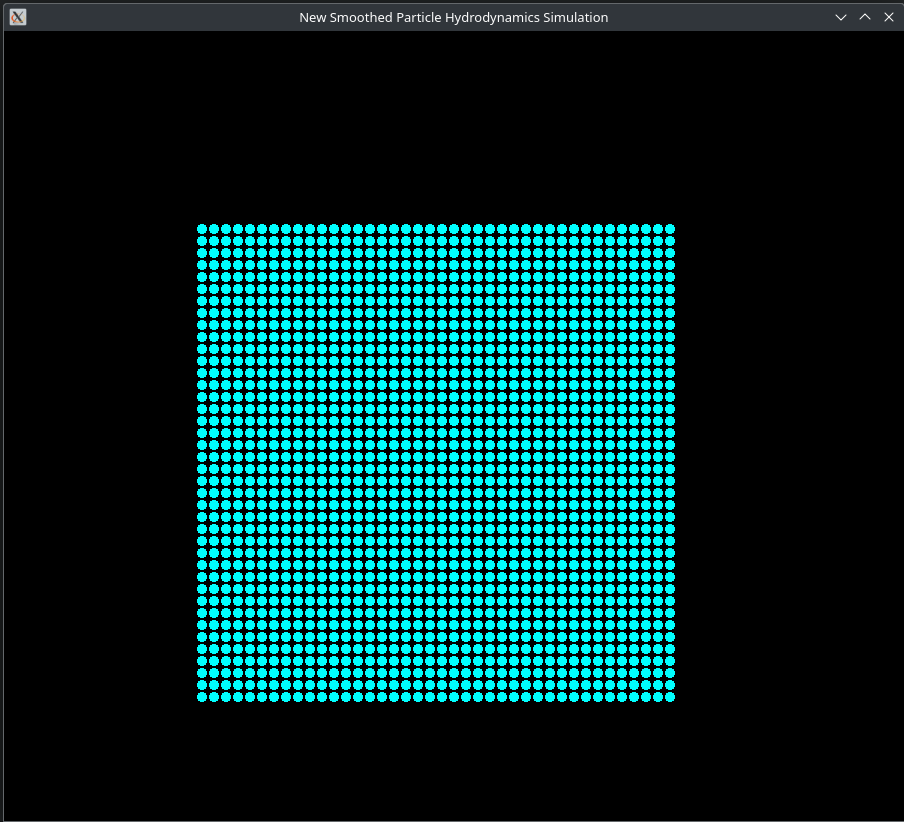
\includegraphics[width=15cm, height=15cm]{more_still_particles_19-05-24}
\caption{Particles placed in an orderly fashion on the screen}
\end{figure}

\subsection{Simulation loop}
In order to calculate new positions of particles, we need to loop over them every step of the simulation to calculate its new position vector using its current velocity and acceleration vectors and multiplying by $dt$, our change in time per simulation step and then draw them. We can begin updating these by implementing gravity first.
\begin{lstlisting}
const float gravity = 9.81f;
const float dt = 1.f/60.f;

 void resolveGravity(int i){
    particles[i].velocity.y += gravity * dt
}
\end{lstlisting}

And within the simulation loop:
\begin{lstlisting}
for (int i = 0; i < particle_num; i++){
    resolveGravity(i);
    particles[i].position.x += particles[i].velocity.x * dt;
    particles[i].position.y += particles[i].velocity.y * dt;
    particles[i].droplet
    .setPosition(particles[i]
    .position.x-particle_radius,
    particles[i].position.y-particle_radius);

    //Draw particles
    window.draw(particles[i].droplet);
\end{lstlisting}
This \href{https://youtube.com/shorts/FSuH_Cs1Qh4?feature=share}{video} shows the implementation of gravity but with no simulation border. This can be implmented with ease in the following manner:

\begin{lstlisting}
void resolveCollisions(int i, sf::Vector2u window_size){
    if (particles[i].position.x > window_size.x || particles[i].position.x < 0){
        particles[i].position.x = clamp((int)particles[i].position.x, 0, (int)window_size.x);
        particles[i].velocity.x *= -1 * collision_damping;
    }
    if (particles[i].position.y >= window_size.y || particles[i].position.y <= 0){
        particles[i].position.y = clamp((int)particles[i].position.y, 0, (int)window_size.y);
        particles[i].velocity.y *= -1 * collision_damping;
    }
}
\end{lstlisting}

I've also implemented a collision damping factor here to simulate the loss the energy upon collision with the simulation border. We now see that we can also successfully interact with the simulation by resizing our window, hitting one of the sucess criteria for this project. The video can be watched \href{https://youtube.com/shorts/wO0xUBSKVck?feature=share}{here}.
\subsection{Predicted Position Optimisation}

The predicted position of the particles, which will be used throughout the development, need to be calculated first. This is done quite easily in this manner:

\begin{lstlisting}
 void predictPositions(int i){
    particles[i].predicted_position.x = particles[i].position.x + particles[i].velocity.x * dt;
    particles[i].predicted_position.y = particles[i].position.y + particles[i].velocity.y * dt;
}
\end{lstlisting}
The function simply predicts the position of the particle depending on the current velocity.


\subsection{Smoothing Kernel and derivative}

As per the theoretical model, my preferred choice of smoothing kernel is the customised version of $W_{\text{spiky}}(r, h)$, allowing for large repulsion forces at small distances and less computationally strenuous powers. In C++, this looks like the following:

\begin{lstlisting}
float smoothingKernel(double dst){
    float volume = pi * (float)(pow(smoothing_radius, 4.0)/2);
    if (dst >=smoothing_radius){
        return 0.f;
    }
    float value = (float)pow(smoothing_radius - dst, 3.0);
    return value/volume;
}
\end{lstlisting}

Notice how we return 0 if the distance is further than the smoothing radius, this saves time as unnecessary values are not computed. The influence value is also divided by the volume of the function, giving us similar influence values regardless of the smoothing radius.

Below is the implementation of the smoothing kernel derivative used for optimisation discussed in the theoretical model.

\begin{lstlisting}
float smoothingKernelDerivative(double dst){
    if (dst >= smoothing_radius) return 0.0;
    float value = -6.f * (smoothing_radius - dst) * (smoothing_radius - dst) / (pi * pow(smoothing_radius, 4));
    return value;
}
\end{lstlisting}

\subsection{Density Calculations}
Calculating the local densities for each point requires us to use the SPH Interpolation equation, $A_s(r) = \sum_{j} m_j \frac{A_j}{\rho_j}W(r-r_j, h)$ \cite{muller}. Interestingly, if we want to calculate the density at a certian point, substituting for $\rho$ gives us:

\begin{center}
 $ \rho_s(r) = \sum_{j} m_j \frac{\rho_j}{\rho_j}W(r-r_j, h),
 \rho_s(r) = \sum_{j} m_j W(r-r_j, h).$
\end{center}
 Where the densities cancel out, giving us a method of calculating the local density without being dependant on it.

\noindent Coding this in C++ gives us:
\begin{lstlisting}
float calculateDensity(int i){
    float density = 0.f;
    for (int j =0; j < particle_num; j++){
        float dst = sqrt();
        //distance is calculated using predicted positions
        float influence = smoothingKernel(dst);
        density += particle_mass * influence;
    }
    return density;
}
\end{lstlisting}

\subsection{Pressure Calculations}
Quantifying the local density into a pressure value, per my theoretical model, would involve taking the local density and finding a pseudo-pressure value, $P_i = k(\rho_i - \rho_0)$ \cite{clavet}, and applying the gradient optimisation to turn this pseudo-pressure into pressure.

The code below is the implementation of the equation above, where $k$ is the pressure multiplier:
\begin{lstlisting}
float densityToPressure(int j){
    float density_error = particles[j].local_density - target_density;
    float local_pressure = density_error * pressure_multiplier;
    return local_pressure;
}
\end{lstlisting}

Then, in order to apply Newton's 3rd law, the index of the 2 particles which are being computing is taken and the average of their pseudo-pressures is returned:

\begin{lstlisting}
 float sharedPressure(int i, int j){
    float pressurei = densityToPressure(particles[i]
    .local_density);
    float pressurej = densityToPressure(particles[j]
    .local_density);
    return (-(pressurei + pressurej) / 2.f);
}
\end{lstlisting}
Notice how a negative pressure value is returned, this ensures pressure is a purely repulsive force which makes intuitive sense as the particles must repel each other.

Finally, the pseudo-pressure is converted to a pressure force using the SPH gradient optimisation which takes into account the rate of change of this property as well as the $x$ and $y$ direction of the particle to turn the scalar pressure force into a vector. Including the nested loop, the implementation of this is below:

\begin{lstlisting}
 sf::Vector2f calculatePressureForce(int i){
    sf::Vector2f pressure_force;
    sf::Vector2f viscosity_force;
    for (int j = 0; j<particle_num; j++){
        if (i == j) continue;
        float x_offset;
        float y_offset;
        if (particles[i].
        predicted_position == particles[j].
        predicted_position){
            x_offset = (float)1+ (rand() % 20);
            y_offset = (float)1+ (rand() % 20);
        }
        else{
            x_offset = particles[j].predicted_position.x - particles[i].predicted_position.x;
            y_offset = particles[j].predicted_position.y - particles[i].predicted_position.y;
        }
        double dst = sqrt(abs(x_offset * x_offset + y_offset * y_offset));
        float gradient = smoothingKernelDerivative(dst);
        float x_dir = x_offset/dst;
        float y_dir = y_offset/dst;
        float shared_pressure = sharedPressure(i, j);
        pressure_force.x += shared_pressure * gradient * particle_mass/particles[j].local_density * x_dir;
        pressure_force.y += shared_pressure * gradient * particle_mass/particles[j]
        .local_density * y_dir;
    }
    return pressure_force;
}
\end{lstlisting}
Notice how a random direction is picked to apply the force if two particles have the same position, this contributes to the particles' Brownian motion.

The returned pressure force must now be converted to an acceleration. This can be done in the main simulation loop by calling the calculatePressureForce function and dividing the value by the density, as per Sebastian Lague's implementation \cite{Lague} of an SPH solver. He mentions this is due to the particles being spheres of volume instead of mass. The implementation within the simulation loop looks like this:

\begin{lstlisting}
sf::Vector2f pressure_force = calculatePressureForce(i);
sf::Vector2f pressure_acceleration;
pressure_acceleration.x = pressure_force.x/particles[i]
.local_density;
pressure_acceleration.y = pressure_force.y/particles[i]
.local_density;
\end{lstlisting}
\subsection{Viscosity}
As calculating viscosity requires a weighted sum from every other particle within the smoothing radius, just like pressure, a nested loop can be used to achieve this. From my theoretical model, implementation in C++ looks like the following:
\begin{lstlisting}

sf::Vector2f calculateViscosityAcceleration(int i){
    sf::Vector2f viscosity_acceleration;
    float dst;
    for (int j; j<particle_num; j++){
        if (i==j) continue;
        float dst;
        //dst is calculated using predicted positions
        viscosity_acceleration.x -= (particles[i].velocity.x - particles[j].velocity.x) * (smoothingKernel(dst)) * viscosity_strength;
        viscosity_acceleration.y -= (particles[i].velocity.y - particles[j].velocity.y) * (smoothingKernel(dst)) * viscosity_strength;
        if (viscosity_acceleration.x > 0 || viscosity_acceleration.y > 0){
            viscosity_acceleration.x = 0;
            viscosity_acceleration.y = 0;
        }
    }
    return viscosity_acceleration;
}

\end{lstlisting}

The acceleration caused by the viscosity within a fluid slows the particle down, this is because viscosity is caused by friction within a fluid, a force which opposes motion. This is why the acceleration casued by viscosity is not added, but rather subtracted from the overall acceleration of the particle.
\subsection{Interactivity and visuals}
One of the criterias for this project is interactivity. Using SFML, I have allowed the user to resize the window but ImGui will allow the user to use sliders and change key SPH properties discussed in this paper such as the Target density, Pressure multiplier and the smoothing radius. Additionally, I will also allow for gravity, number of particles and particle mass to also be changed to allow the user freedom and to explore different types of fluid which are possible to simulate using this technique. ImGui interactive variable initialisation code is below:

\begin{lstlisting}
ImGui::Begin("Menu");
ImGui::SliderInt("Particle Num", &particle_num, 1, 1600);
ImGui::SliderFloat("Particle Mass", &particle_mass, 0.1f, 100.f);
ImGui::SliderFloat("Target Density", &target_density, 0.f, 500.f);
ImGui::SliderFloat("Pressure Multiplier", &pressure_multiplier, 0.f, 1000.f);
ImGui::SliderFloat("Smoothing Radius", &smoothing_radius, 10, 200);
ImGui::SliderFloat("Gravity", &gravity, 0.f, 100.f);
ImGui::SliderInt("Framerate", &framerate, 60, 1200);
ImGui::End();
\end{lstlisting}

In terms of the visuals of the project, cyan particles were being rendered earlier. Instead, a more aesthetically pleasing and useful algorithm to implement would be a linear interpolation colour algorithm. Simply put, the algorithm would output a colour for the particle depending on it's velocity. A larger velocity would output a more red-shifted colour whereas a slower velocity would output a blue-shifted colour. In C++, we would have:

\begin{lstlisting}
 void resolveColor(int i, float vel){
    int b = clamp((int)(-255/50 * vel + 255), 0, 255);
    int r = clamp((int)(255/50 * vel -255), 0, 255);
    int g = clamp((int)(-abs(255/50 * (vel-50))+255), 0, 255);
    particles[i].droplet.setFillColor
    (sf::Color(r, g, b));
}
\end{lstlisting}
This will be run in the simulation loop after the velocities have been calculated for all particles in that frame. The intention behind this is to be able to better explain densities by visualising them, as well as evaluate any anomalies within the simulation.
\subsection{Updating Simulation loop}
Finally, we can accumulate update our simulation loop by putting together everything within our development so far. This is the updated simulation loop:

\begin{lstlisting}
 for (int i = 0; i < particle_num; i++){
    resolveCollisions(i, window_size);
    //gravity step
    resolveGravity(i);
    //Predict next positions
    predictPositions(i);
    // window bounding box
    //calculate densities
    particles[i].local_density = calculateDensity(i);
    //convert density to pressure
    particles[i].local_pressure = densityToPressure(i);
    //Calculate pressure forces and acceleration
    sf::Vector2f pressure_force = calculatePressureForce(i);
    sf::Vector2f pressure_acceleration;
    pressure_acceleration.x = pressure_force.x/particles[i].local_density;
    pressure_acceleration.y = pressure_force.y/particles[i].local_density;
    //Calculate acceleration due to viscosity
    pressure_acceleration += calculateViscosityAcceleration(i);
    //calculate velocity
    particles[i].velocity.x += pressure_acceleration.x * dt;
    particles[i].velocity.y += pressure_acceleration.y * dt;
    //resolve colour
    float vel = sqrt(particles[i].velocity.x * particles[i].velocity.x + particles[i].velocity.y * particles[i].velocity.y);
    resolveColour(i, vel);
    //calculate particle positions with radius offset
    particles[i].position.x += particles[i].velocity.x * dt;
    particles[i].position.y += particles[i].velocity.y * dt;
    //set particle position on screen
    particles[i].droplet.setPosition
    (particles[i].position.x+particle_radius, particles[i].position.y+particle_radius);
    //render particle
    window.draw(particles[i].droplet);
}
\end{lstlisting}
\subsection{Final Product}

\end{document}
